
\section{Filter-Umwandlungen mittels Frequenztransformation}
\label{Frequenztransformation}

\subsection{Transformation: Tiefpass -- Hochpass}{344}

In der Übertragungsfunktion des Tiefpasses werden alle $S$ durch $\frac{1}{S}$ ersetzt

\begin{minipage}[c]{0.4\columnwidth}
    $$ \boxed{H_{\rm HP}(S) = H_{\rm TP} \Bigg(\frac{1}{S} \Bigg) } $$
\end{minipage}
\hfill
\begin{minipage}[c]{0.58\columnwidth}
    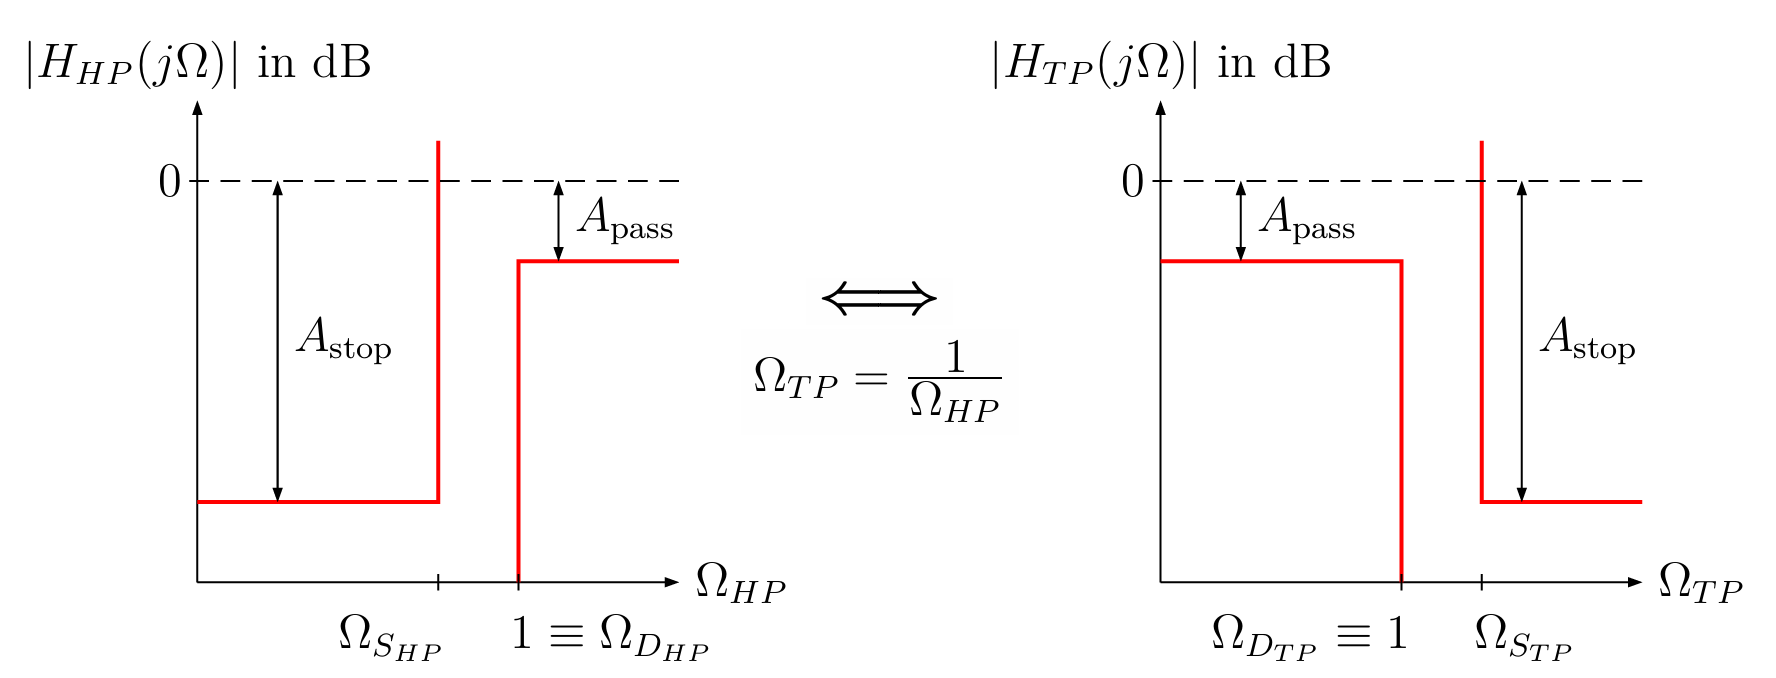
\includegraphics[width=\columnwidth]{images/toleranzschema_HP_TP.png}
\end{minipage}

\vspace{0.2cm}
Zwischen allen normierten Frequenzen, im Speziellen den normierten \textbf{Eckfrequenzen} der \textbf{Sperrbereiche}
$\Omega_{S_{\rm TP}}$ und $\Omega_{S_{\rm HP}}$ und \textbf{Durchlassbereiche} $\Omega_{D_{\rm TP}}$ und $\Omega_{D_{\rm HP}}$ gilt:
$$ \boxed{ \Omega_{S_{\rm TP}} = \frac{1}{\Omega_{S_{\rm HP}}}  \qquad 1 = \Omega_{D_{\rm TP}} = \frac{1}{\Omega_{D_{\rm HP}}} } $$


\begin{minipage}[t]{0.48\columnwidth}
    \subsubsection{Bauteiltransformationen}

    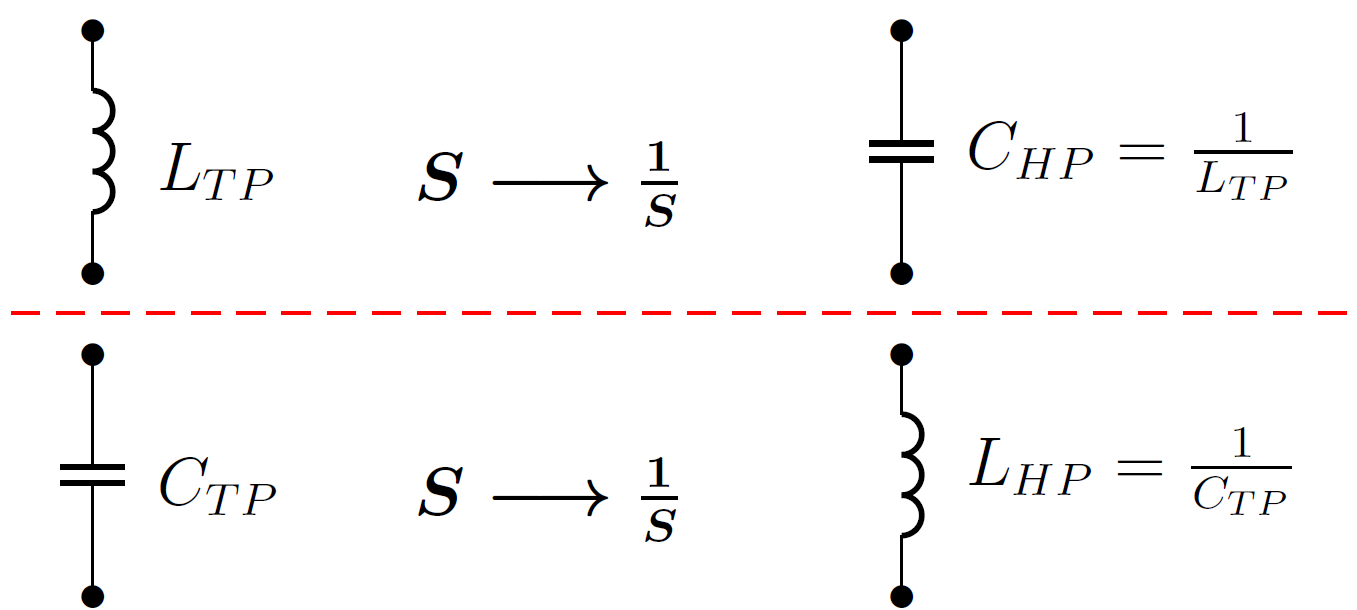
\includegraphics[width=\columnwidth]{images/bauteiltransformation_TP_HP.png}
\end{minipage}
\hfill
\begin{minipage}[t]{0.48\columnwidth}
    \subsubsection{Singularitäten}

    \begin{tabular}{ll}
        Pole:           & $P_{k, \rm HP} = \frac{1}{P_{k, \rm TP}}$ \\
        Nullstellen:    & $Z_{i, \rm HP} = \frac{1}{Z_{i, \rm TP}}$ \\
        \\
    \end{tabular}

    \textbf{\textrightarrow\ Polgüte bleibt erhalten}
\end{minipage}


\subsection{Transformation: Tiefpass -- Bandpass}{348}

In der Übertragungsfunktion des Tiefpasses werden alle $S$ durch $\frac{S^2  + 1}{B \cdot S}$ ersetzt, wobei $B$ der normierten
Bandbreite entspricht. \\
\textbf{Voraussetzung:} $\omega_r = \sqrt{\omega_{B1} \cdot \omega_{B2}} = \sqrt{\omega_{S1} \cdot \omega_{S2} } $\\
Sollte diese Voraussetzung nicht erfüllt sein, muss sie erfüllt werden, indem das Toleranzschema 'strenger' ausgelegt wird.

\begin{minipage}[c]{0.4\columnwidth}
    $$ \boxed{H_{\rm BP}(S) = H_{\rm TP} \Bigg(\frac{S^2  + 1}{B \cdot S} \Bigg) } $$
    $$ \boxed{ B = \frac{\omega_{B2} - \omega_{B1}}{\omega_r} = \Omega_{B2} - \Omega_{B1} } $$
\end{minipage}
\hfill
\begin{minipage}[c]{0.58\columnwidth}
    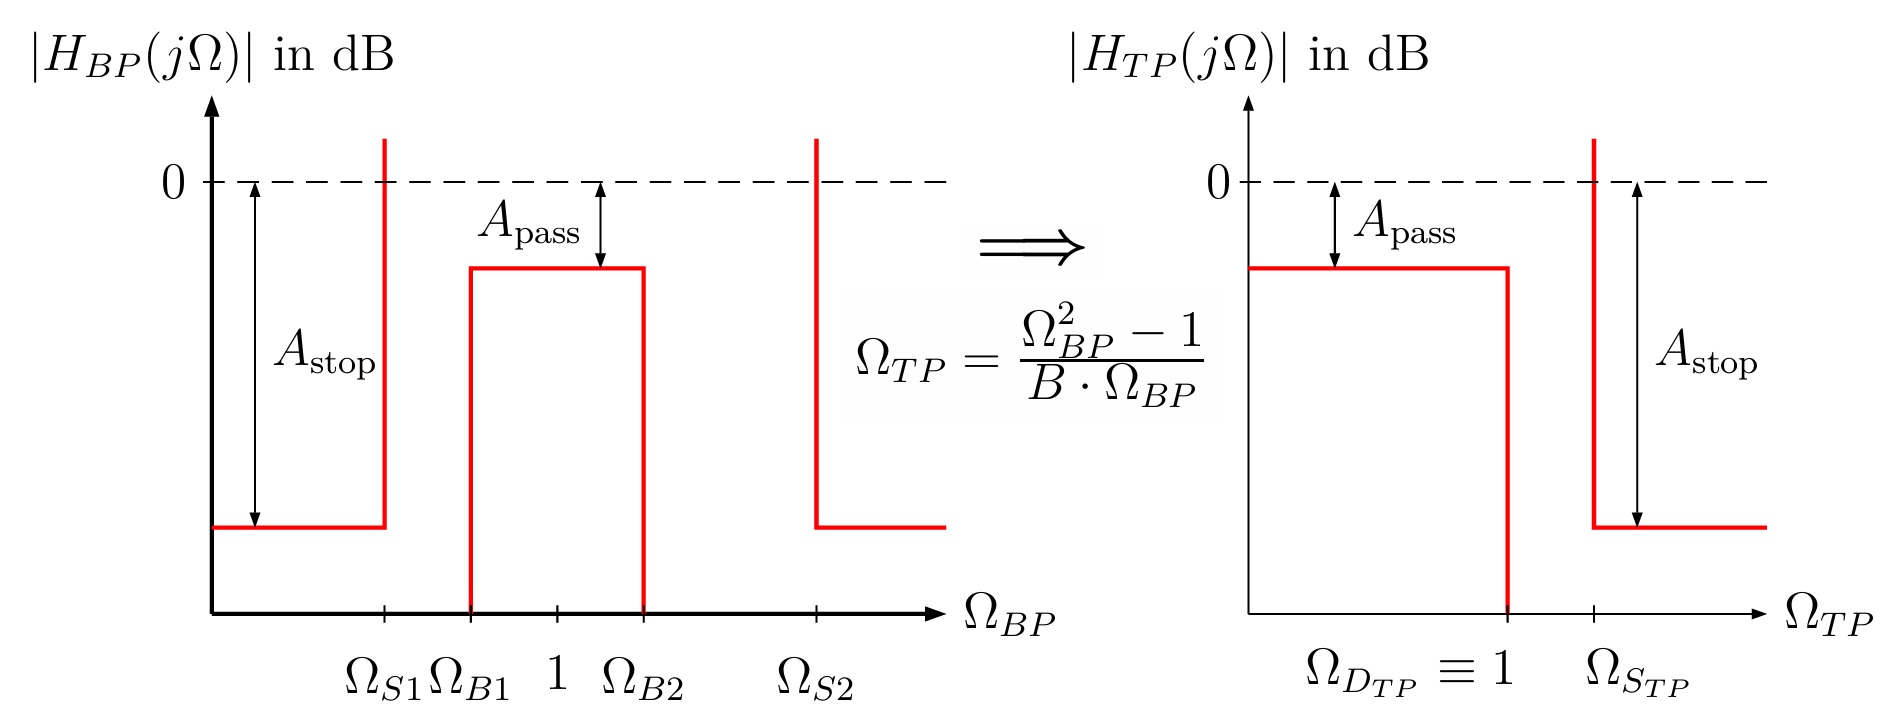
\includegraphics[width=\columnwidth]{images/toleranzschema_BP_TP.png}
\end{minipage}

\vspace{0.2cm}
Zwischen allen normierten Frequenzen $\Omega_{S_{\rm TP}}$, $\Omega_{S1}$, $\Omega_{S2}$, $\Omega_{B1}$ und $\Omega_B2$ gilt:
$$ \boxed{ \Omega_{S_{\rm TP}} = \frac{\Omega_{S2} - \Omega_{S1}}{B} = \frac{\Omega_{S2} - \Omega_{S1}}{\Omega_{B2} - \Omega_{B1}}
    = \frac{\omega_{S2} - \omega_{S1}}{\omega_{B2} - \omega_{B1}} = \frac{f_{S2} - f_{S1}}{f_{B2} - f_{B1}} } $$

\textbf{Hinweis: Die Transformation erhöht die Filterordnung um Faktor 2}


\begin{minipage}[t]{0.48\columnwidth}
    \subsubsection{Bauteiltransformationen}

    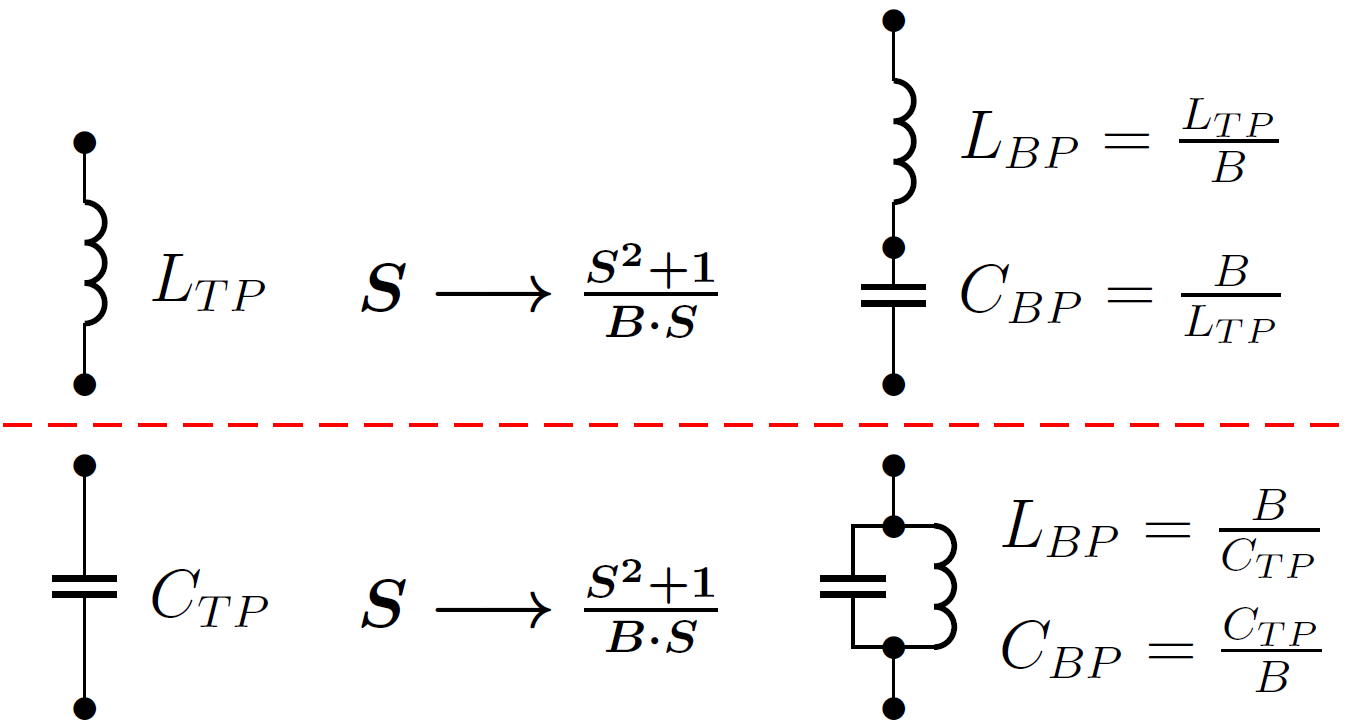
\includegraphics[width=\columnwidth]{images/bauteiltransformation_TP_BP.png}
\end{minipage}
\hfill
\begin{minipage}[t]{0.48\columnwidth}
    \subsubsection{Singularitäten}

    \textrightarrow\ Siehe Skript S. 351-352
\end{minipage}



\subsection{Transformation: Tiefpass -- Bandsperre}{357}

In der Übertragungsfunktion des Tiefpasses werden alle $S$ durch $\frac{B \cdot S}{S^2 + 1}$ ersetzt, wobei $B$ der normierten
Bandbreite entspricht. \\
\textbf{Voraussetzung:} $\omega_r = \sqrt{\omega_{B1} \cdot \omega_{B2}} = \sqrt{\omega_{S1} \cdot \omega_{S2} } $\\
Sollte diese Voraussetzung nicht erfüllt sein, muss sie erfüllt werden, indem das Toleranzschema 'strenger' ausgelegt wird.

\begin{minipage}[c]{0.4\columnwidth}
    $$ \boxed{H_{\rm BP}(S) = H_{\rm TP} \Bigg(\frac{B \cdot S}{S^2 + 1} \Bigg) } $$
    $$ \boxed{ B = \frac{\omega_{B2} - \omega_{B1}}{\omega_r} = \Omega_{B2} - \Omega_{B1} } $$
\end{minipage}
\hfill
\begin{minipage}[c]{0.58\columnwidth}
    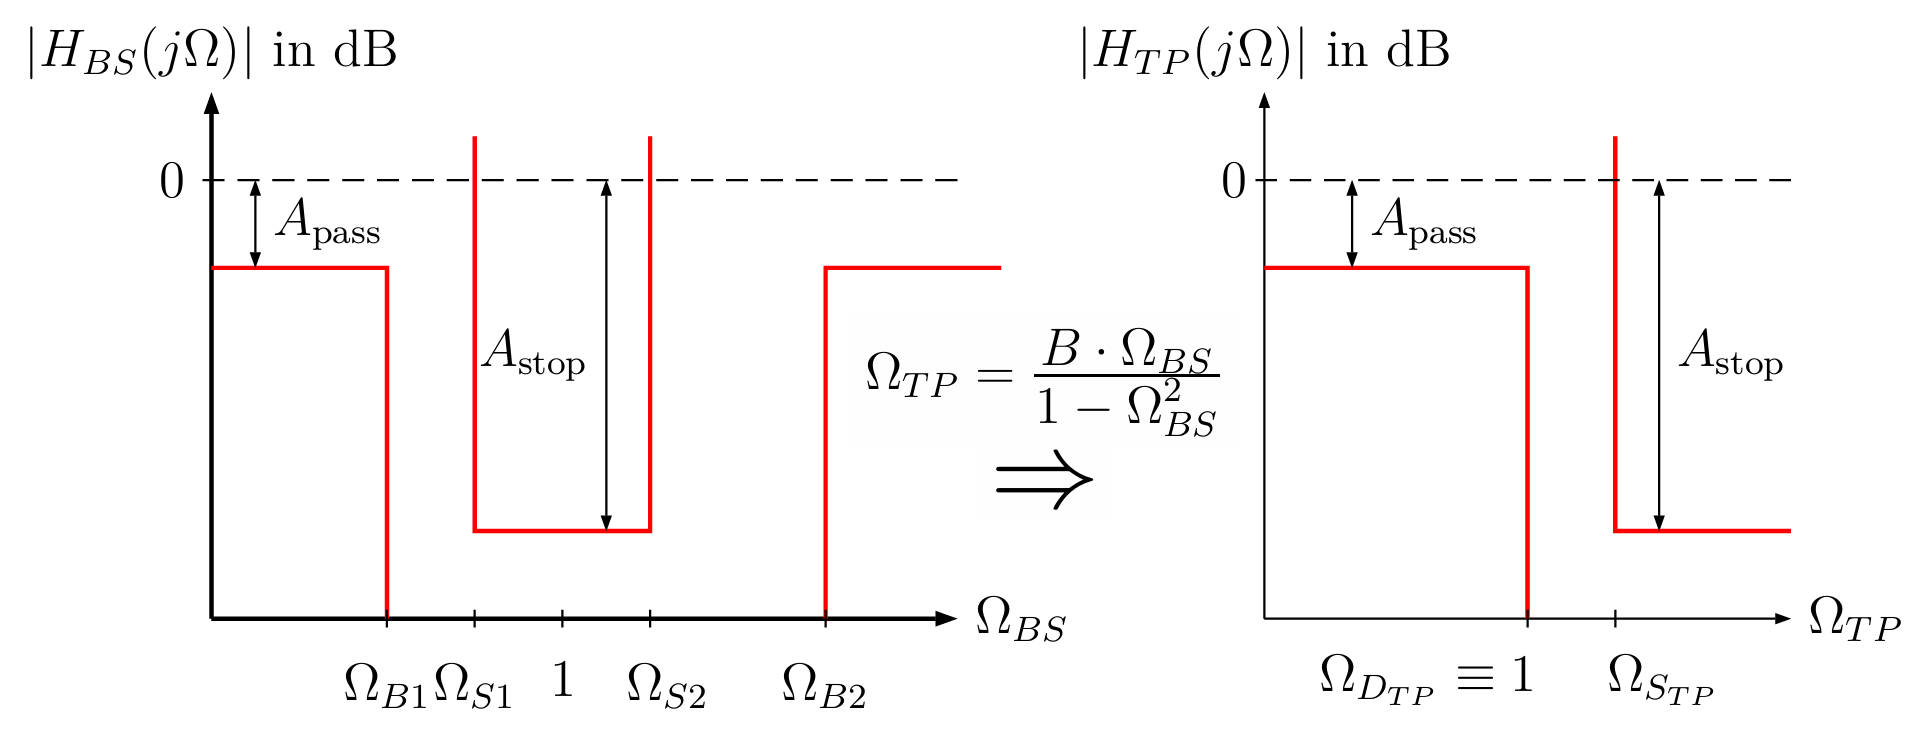
\includegraphics[width=\columnwidth]{images/toleranzschema_BS_TP.png}
\end{minipage}

\vspace{0.2cm}
Zwischen allen normierten Frequenzen $\Omega_{S_{\rm TP}}$, $\Omega_{S1}$, $\Omega_{S2}$, $\Omega_{B1}$ und $\Omega_B2$ gilt:
$$ \boxed{ \Omega_{S_{\rm TP}} = \frac{B}{\Omega_{S2} - \Omega_{S1}} = \frac{\Omega_{B2} - \Omega_{B1}}{\Omega_{S2} - \Omega_{S1}}
    = \frac{\omega_{B2} - \omega_{B1}}{\omega_{S2} - \omega_{S1}} = \frac{f_{B2} - f_{B1}}{f_{S2} - f_{S1}} } $$

\textbf{Hinweis: Die Transformation erhöht die Filterordnung um Faktor 2}


\begin{minipage}[t]{0.48\columnwidth}
    \subsubsection{Bauteiltransformationen}
    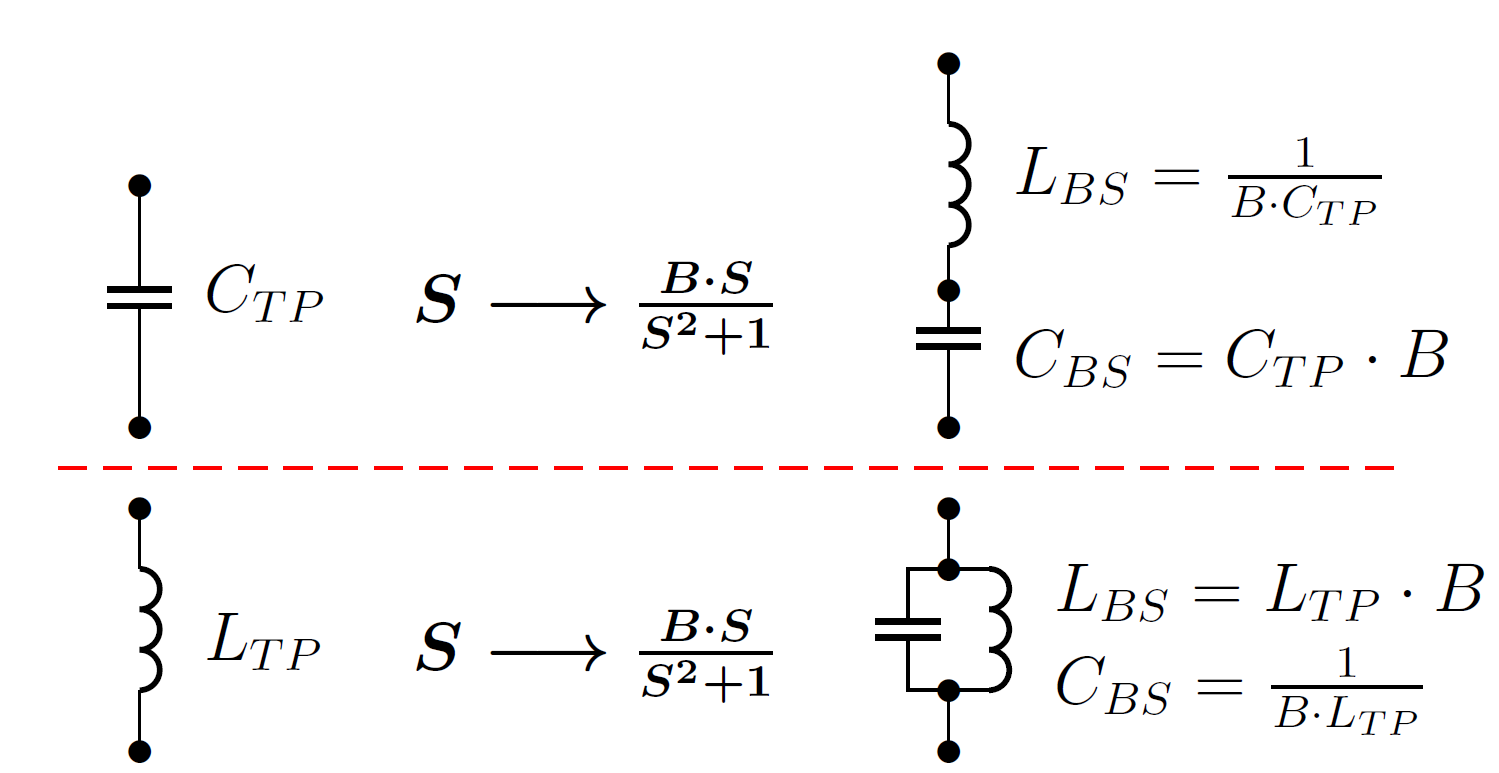
\includegraphics[width=\columnwidth]{images/bauteiltransformation_TP_BS.png}
\end{minipage}
\hfill
\begin{minipage}[t]{0.48\columnwidth}
    \subsubsection{Singularitäten}

    \textrightarrow\ Siehe Skript S.359
\end{minipage}
